%%%%%%%%%%%%%%%%%%%%%%%%%%%%%%%%%%%%%%%%%%%%%%%%%%%%%%%%%%%%%%%%%%%%%%%%%
% Angaben zur Person
%%%%%%%%%%%%%%%%%%%%%%%%%%%%%%%%%%%%%%%%%%%%%%%%%%%%%%%%%%%%%%%%%%%%%%%%%
\newcommand{\name}{Dennis Pidun}
\newcommand{\matr}{??????}
\newcommand{\email}{pidund@uni-hildesheim.de}
\newcommand{\studgang}{Angewandte Informatik (B.Sc.)}
\newcommand{\thema}{Safety Engineering in AGI}
\newcommand{\keywords}{}
\newcommand{\betreuer}{Dr. Pascal Reuß}

%%%%%%%%%%%%%%%%%%%%%%%%%%%%%%%%%%%%%%%%%%%%%%%%%%%%%%%%%%%%%%%%%%%%%%%%%
% Angaben zum Seminar
%%%%%%%%%%%%%%%%%%%%%%%%%%%%%%%%%%%%%%%%%%%%%%%%%%%%%%%%%%%%%%%%%%%%%%%%%
\newcommand{\semester}{Wintersemester 2019/2020}
\newcommand{\vtyp}{Seminar}
\newcommand{\veranstaltung}{IIS Seminar}
\newcommand{\prof}{Prof. Dr. Klaus-Dieter Althoff}
\newcommand{\lehrstuhl}{Institut für Informatik\\Bereich Intelligente Informationssysteme}

%%%%%%%%%%%%%%%%%%%%%%%%%%%%%%%%%%%%%%%%%%%%%%%%%%%%%%%%%%%
%% Diese Datei sollten Sie nicht anpassen, sie definiert %%
%% ein Dokument der Form, in der wir es erwarten.        %%
%%%%%%%%%%%%%%%%%%%%%%%%%%%%%%%%%%%%%%%%%%%%%%%%%%%%%%%%%%%

%Schriftgr��e, ein- oder zweiseitig, Papierformat, Dokumententyp
\documentclass[12pt,oneside,a4paper]{scrartcl}

\usepackage[latin1]{inputenc}
%Seitenr�nder
\usepackage[left=2.5cm,right=2.5cm,top=2.5cm,bottom=2cm]{geometry}

%NDR und Umlaute
\usepackage{ngerman}
\usepackage[latin1]{inputenc}

%Kopf- und Fu�zeile
\usepackage{fancyhdr}
\pagestyle{fancy}
\fancyhf{}

%Kopfzeile links bzw. innen
\fancyhead[L]{\name}

%Kopfzeile mittig
\fancyhead[C]{\thepage}

%Kopfzeile rechts bzw. au�en
\fancyhead[R]{\thema}

%Linie oben
\renewcommand{\headrulewidth}{0.5pt}

%F�r farbige Links
\usepackage{color}

%H�bsche Schriften im PDF-Viewer
\usepackage{ae}
\usepackage{times}

% Brauchbare PDF-Links und angaben im PDF-Header
\usepackage[pdftex,
 raiselinks=true,%
  bookmarks=true,%
  colorlinks=false,% Gibt man keine gedruckte Version ab, sondern das PDF, sollte man erw�gen diesesn Wert auf "true" zu �ndern
  bookmarksopenlevel=1,%
  bookmarksopen=true,%
  bookmarksnumbered=true,%
  hyperindex=true,% 
  plainpages=false,% correct hyperlinks
  pdfpagelabels=true,% view TeX pagenumber in PDF reader
 pdfstartview=FitH]{hyperref}
%%  pdfborder={0 0 0.5}
 %%  pdfauthor={\name},
%%  pdfsubject={\veranstaltung},
%%  pdfkeywords={\keywords},
%%  pdftitle={\thema},
 
%Thumbnails im PDF
\usepackage{thumbpdf}

%h�bschere Tabellenabst�nde
\usepackage{booktabs}

%diverser mathematischer Kram
\usepackage{amsmath}

% F�r den dinat zitier stil
\usepackage{natbib}

% Graphiken
\usepackage[final]{graphicx}

% Verhindern von "Schusterjungen" und "Hurenkindern"
\clubpenalty = 10000
\widowpenalty = 10000
\displaywidowpenalty = 10000
\tolerance=500 %Zeilenumbruch




\usepackage[utf8]{inputenc}
\usepackage[T1]{fontenc}

%%%%%%%%%%%%%%%%%%%%%%%%%%%%%%%%%%%%%%%%%%%%%%%%%%%%%%%%%%%%%%%%%%%%%%%%%
% Zusatzpakete
%%%%%%%%%%%%%%%%%%%%%%%%%%%%%%%%%%%%%%%%%%%%%%%%%%%%%%%%%%%%%%%%%%%%%%%%%

\begin{document}
%%%%%%%%%%%%%%%%%%%%%%%%%%%%%%%%%%%%%%%%%%%%%%%%%%%%%%%%%%
%% Dies hier ist die Titelseite.                        %%
%% Auch hier brauchen sie KEINE �nderungen vorzunehmen! %%
%% Die entsprechenden Angaben werden aus den Variablen  %%
%% in IIS-Seminar-Vorlage.tex �bernommen.               %%
%%%%%%%%%%%%%%%%%%%%%%%%%%%%%%%%%%%%%%%%%%%%%%%%%%%%%%%%%%

\thispagestyle{empty}
\linespread {1.25}\selectfont % eineinhalbfachen Zeilenabstand f�r diesen Block
\begin{flushright}
Universit\"at Hildesheim\\
\lehrstuhl\\
\prof\\
\end{flushright}
\begin{center}
\linespread {1.05}\selectfont % 1.25-facher Zeilenabstand
\vfill
\LARGE{\vtyp\\*[.1cm]\parbox{0.6\textwidth}{\begin{center}\veranstaltung\end{center}}\\*[.2cm]}
\large{\textbf{Thema: \thema\\~\\}
Betreuer: \betreuer\\~\\
\semester}
\vfill
\name\\
Matrikelnummer: \matr\\
Studiengang: \studgang\\~\\
E-Mail: \href{mailto:\email}{\email}\\
\end{center}
% R�cksetzen des Seitenz�hlers
\setcounter{page}{0}
\newpage


%%%%%%%%%%%%%%%%%%%%%%%%%%%%%%%%%%%%%%%%%%%%%%%%%%%%%%%%%%%%%%%%%%%%%%%%%
% Abstract etc.
%%%%%%%%%%%%%%%%%%%%%%%%%%%%%%%%%%%%%%%%%%%%%%%%%%%%%%%%%%%%%%%%%%%%%%%%%
\section*{Abstract}
\begin{abstract}\textsl{
Abstract einfügen.
}\end{abstract}
\newpage

%%%%%%%%%%%%%%%%%%%%%%%%%%%%%%%%%%%%%%%%%%%%%%%%%%%%%%%%%%%%%%%%%%%%%%%%%
% Inhaltsverzeichnis
%%%%%%%%%%%%%%%%%%%%%%%%%%%%%%%%%%%%%%%%%%%%%%%%%%%%%%%%%%%%%%%%%%%%%%%%%
\tableofcontents

%%%%%%%%%%%%%%%%%%%%%%%%%%%%%%%%%%%%%%%%%%%%%%%%%%%%%%%%%%%%%%%%%%%%%%%%%
% Inhalt
%%%%%%%%%%%%%%%%%%%%%%%%%%%%%%%%%%%%%%%%%%%%%%%%%%%%%%%%%%%%%%%%%%%%%%%%%

\section{Einführung}
    \subsection{Motivation}
    Die Technologien im Bereich der künstlichen Intelligenz sind ständig im Wandel. Tag für Tag
    werden daher immer wieder neue Entdeckungen gemacht, welche es ermöglichen schwierige Probleme
    in simplen Schritten zu lösen. Dabei wird die Forschung ständig vor neuen Herausforderungen
    gestellt, nicht nur werden Abläufe und Prozesse immer schneller, es treten auch Probleme auf,
    welche es gilt zu identifizieren und im besten Fall vorzubeugen. Diese Arbeit zielt daher
    darauf ab Konzepte herauszufinden, welche es ermöglichen möglichst gezielt für Sicherheit
    in der Entwicklung von Artificial General Intelligence zu sorgen. Die Herausforderung eine
    sichere Umgebung sowohl für Mensch als auch für die Maschine aufzustellen, stellt somit das
    Kernthema dar. //TBC

    \subsection{Machine Ethics}
    //Überarbeiten//    
    Um die Frage, warum Machine Ethics wichtig sind zu klären, stellen wir uns zunächst ein
    Scenario vor, welches bereits Patrick Lin \cite[p. 70]{maurer_gerdes_lenz_winner_2015}
    aufgestellt wurde. Hierbei handelt es sich um eine Situation, welche bereits heute auf den
    Straßen auftreten kann. Um die moralischen Entscheidungen in dem Prozess des Fahrens zu
    verdeutlichen, stellen wir uns also vor, dass man in einem Auto sitzt und nun eine 
    Entscheidung treffen muss. Nämlich die Entscheidung, ob man nach links ausweicht und damit
    ein junges Mädchen umbringt oder ob man nach rechts ausweicht und damit eine ältere 
    Seniorin umbringt. Weicht man nicht aus, werden augenblicklich beide Menschen mit in den
    Tot gerissen. Dieses Beispiel ist tatsächlich sehr dramatisch gewählt, was jedoch sehr gut
    verdeutlicht, welche nicht rationalen Entscheidungen getroffen werden müssen. Egal welche 
    Entscheidung hierbei getroffen wird, am Ende stirbt mindestens ein Mensch, was in jeder 
    Hinsicht einen Verlust darstellt und ohnehin moralisch nicht korrekt wäre. \cite[p. 70]{maurer_gerdes_lenz_winner_2015}
    Mit seiner Entscheidung kann man letztendlich nur bestimmen, welche Person benachteiligt 
    wird. In einer solchen Situation jedoch hätte der Mensch ohnehin keine Zeit diese Entscheidung
    rational zu betrachten. Ferner hätte der Mensch ebenfalls nicht die Möglichkeiten und 
    das Wissen gerecht zu entscheiden.
    //Überarbeiten// 
    
    Ein weiteres Problem ist außerdem, dass man nicht genau weiß, welche moralischen Werte man
    innerhalb der AGI verankern soll. \cite[p. 1]{yampolskiy2013safety} Es wird daher viel 
    diskutiert, welche moralischen Wertvorstellungen die richtigen sind. In diversen Literaturen
    findet man unter verschiedenen Titeln immer wieder Diskussionen, welche sich genau mit dieser
    Fragestellung auseinandersetzen. Yampolskiy spricht hier davon, dass keine effektiven 
    Maßnahmen getroffen werden, da sich einerseits viel damit beschäftigt wird, sich andererseits 
    aber nichts wandelt und kein nutzbares Ergebnis herauskommt \cite[p. 1]{yampolskiy2013safety}.
    Dies greifen Yampolskiy und Fox nun auf, um über verschiedene Möglichkeiten dieses Problem zu
    lösen zu diskutieren. 
    
    Laut Yampolskiy und Fox stellt man sich diese Fragen nicht nur bei near-human-AIs, sondern 
    ebenso bei superintelligent AIs \cite[p. 2]{yampolskiy2013safety}. Es ist ferner deutlich 
    bedeutender, so Fox und Yampolskiy, dass man sich gerade im Hinblick auf die immer schnelleren
    Fortschritte in AGIs, Gedanken um die Sicherheit und Moral bei superintelligent AIs macht. 
    So gehen Crnkovic und {\c{C}}{\"u}r{\"u}kl{\"u} in \cite[p. 1]{crnkovic2012robots} ebenfalls
    davon aus, dass die Betrachtung der Moral in superintelligent AIs eine übergeordnete Rolle 
    haben muss. Sie sprechen hier davon, dass AIs genau das tun würden, wozu sie programmiert 
    wurden, was jedoch nicht exakt richtig ist. Hierbei muss man nämlich zwischen simplen Agenten 
    und komplexeren Agentensystemen unterscheiden, da mit steigender Komplexität und erhöter 
    Autonomität die moralischen Herausforderungen ebenfalls ansteigen werden. Crnkovic et al
    stellen hier den folgenden Grundsatz auf: ``intelligence must come in conjunction with ethics,
    through the concept of an artifact ethical by design''. Um dies zu unterstützen, gehe ich daher
    auf die Möglichkeiten im Bereich des Safety Engineerings ein.
    
\section{Artificial General Intelligence}
    Um besser differenzieren zu können, um welche Art von künstlicher Intelligenz hier behandelt 
    wird, werde ich nachfolgend auf diverse Definitionen eingehen, welche sich mit den verschiedenen
    Stufen von AI(-Systemen) und deren Abgrenzung beschäftigen. 
    
    \subsection{Classical Artificial Intelligence}\label{subsec:cai}
    John McCarthy stellte zu Beginn der Era der künstlichen Intelligenz bereits folgende Definition
    auf: ``Getting a computer to do things which, when done by people, are said to involve intelligence.'' 
    \cite[p. 1]{ertel2016grundkurs}. Dies ist jedoch eine sehr allgemeine Definition für das 
    Verhalten von Maschinen, die über künstliche Intelligenz verfügen sollen. Daher stelle ich mir 
    diverse Fragen dazu, unter Anderem: ``Was ist Intelligenz?'', ``Wie kann eine Maschine intelligentes
    Verhalten zeigen?'' und ``Wann gilt eine Maschine als intelligent?''. All diese Fragen sind die 
    Grundlage für eine intelligente Maschine, welche eigenständig nach Lösungswegen für ein spezielles
    Problem suchen. Um dies zu testen, stellt Ertel folgende Situation auf: Man stelle sich ein Feld 
    vor, auf dem Roboter wild um herzufahren scheinen. Einige folgen einander, andere weichen einander 
    aus, wieder andere haben keine klaren Ziele. \cite[p. 2]{ertel2016grundkurs} Ertel stellt hier die
    Frage ``Sehen wir hier intelligentes Verhalten?'', wobei nach Definition von McCarthy hier von 
    intelligentem Verhalten gesprochen werden kann. In \ref{pic:braitenberg-vehikel} sieht man zwei 
    simple Verschaltungen dieser sogenannten Breitenberg-Vehikel. Dargestellt werden hier simple 
    Verschaltungen von Sensoren zu Motoren, welche je nach Lichtstärke unterschiedlich reagieren. 
    Man kann nun diskutieren, ob dieses Verhalten wirklich ein intelligentes Verhalten ist oder
    nur durch Zufall intelligent erscheint. Ertel behauptet daher, dass die obige Definition nicht
    ausreichend ist, da KI sich zum Ziel setzt, viele schwierige Probleme zu lösen. In diesem Beispiel
    wären die Braitenberg-Vehikel mit anderen komplexeren Situationen sichtlich überfordert.
    
    \begin{figure}[h]\begin{center}
        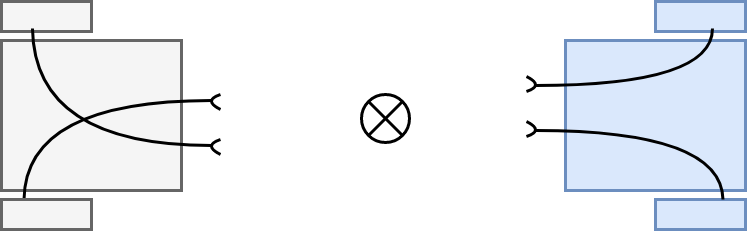
\includegraphics[width=0.8\textwidth]{figures/braitenberg-roboter.png}
        \caption[Verschaltung Braitenberg-Vehikel]{Simple Verschaltung zweier Braitenbergvehikel nach \cite{ertel2016grundkurs}}
        \label{pic:braitenberg-vehikel}
    \end{center}\end{figure}
    
    Die Aussage von John McCarthy ist schlichtweg nicht genau genug und bestimmt nicht im Detail was
    genau Intelligenz bedeutet. Dabei besteht Intelligenz laut Shukla et al. aus zwei Grundkomponenten: 
    Zunächst benötigt man die Fähigkeit neue Konzepte zu erlernen, sprich Informationen nicht nur 
    aufzunehmen sondern auch zu verarbeiten und in Wissen umzuwandeln. Dieses Wissen muss außerdem 
    korrekt angewendet werden, woraus insgesamt Schlussfolgerungen über die reale Welt gezogen werden 
    können. \cite{shukla2013applicability} Bei den Braitenberg Vehikeln ist dies jedoch nicht der Fall,
    alles was sie tun ist eine Information - hier die Lichtstärke der Lichtquelle - aufnehmen und diese
    in mechanische Energie - also die Bewegung eines Motors - umzuwandeln. Man kann hier allerdings nicht
    von Wissen sprechen, da hier keine Informationen erlernt oder in irgendeiner Weise abgelegt werden.
    
    Um nun zu verstehen, warum man bei intelligenten Maschinen davon spricht, dass sie über eine 
    künstliche Intelligenz verfügen, muss man sich vor Augen halten in welchen Gebieten diese Maschinen
    eingesetzt werden sollen. Unteranderem werden diese künstlichen Intelligenzen in Bereichen eingesetzt,
    wo es die Situation erfordert, dass die menschliche Intelligenz Unterstützung erfahren muss
    \cite[p. 2]{ertel2016grundkurs}. Diese Bereiche sind in jedem Fall speziell und nicht im Generellen
    zu verstehen. Bei künstlicher Intelligenz kann man daher festhalten, dass sie sich auf bestimmte Bereiche
    konzentriert und dort generalisierend wirkt. Elaine Rich hielt daher fest: ``Artificial Intelligence
    is the study of how to make computers do things at which, at the moment, people are better.''.
    Beispielsweise sind (normale) Computer sehr gut darin Berechnungen in Bruchteilen durchzuführen und
    diese zu Ergebnissen zu führen \cite[p. 3]{ertel2016grundkurs}. In anderen Bereichen schneiden
    dahingegen diese Computer wiederum schlecht ab. Abhilfe, so Ertel, könnten daher künstliche Intelligenzen
    in Form von neuronalen Netzen sein.

    \subsection{Verbindung zu ''Strong AI''}
    Viele Quellen berichten, dass man grundsätzlich zwischen Strong AI und Weak AI unterscheidet
    \cite{huang_beef}. Doch war sind die Bedingungen um eine Künstliche Intelligenz in die Kategorien
    ``Weak'' und ``Strong'' zu unterteilen?

    Schwache KIs sind, wie wir bereits in \ref{subsec:cai} kennengelernt haben, Systeme welche genau auf
    eine Anwendung hin konzipiert und trainiert wurden. Diese schwachen Systeme beziehungsweise schwach
    intelligente Maschinen stellen dabei den Großteil in der aktuellen Entwicklung dar \city{brendel_2019}.
    Aber wie groß ist der Schritt um von einer Weak, beziehungsweise schwachen KI zu einer Strong,
    beziehungsweise starken KI zu gelangen?


    \subsection{Aktueller Forschungsstand bei AGI-Systems}
    
\section{Safety Engineering}
    \subsection{Probleme bei AI Engineering}
    \subsection{AI Safety in klassischen AI Systems}
    \subsection{AI Safety in Artificial Superintelligent Systems}

%% Eher nochmal bearbeiten:
    \subsection{Problemlösungsansätze} 
    \subsection{Simulated Areas / Simulations}
\section{The Artificial Confinementproblem}
    \subsection{Kritik des Confinement Approach}
    \subsection{Mögliche Escape Paths}
    \subsection{Social Engineering Attacks}
\section{AI Boxing Strategies}
    \subsection{Physical Boxing}
    \subsection{Psychological Boxing}
    \subsection{Kombination mit anderen Limitierungstechniken}
\section{Fazit}

\newpage
%%%%%%%%%%%%%%%%%%%%%%%%%%%%%%%%%%%%%%%%%%%%%%%%%%%%%%%%%%%%%%%%%%%%%%%%%
%% Einbinden der Quellen
%% https://www.overleaf.com/learn/latex/Bibliography_management_with_bibtex#Reference_guide
%%%%%%%%%%%%%%%%%%%%%%%%%%%%%%%%%%%%%%%%%%%%%%%%%%%%%%%%%%%%%%%%%%%%%%%%%
\addcontentsline{toc}{section}{\bibname}
\bibliography{quellen}
\bibliographystyle{dinat}

\listoffigures

\end{document}
